\newpage

\section{Destruição de dados}

Conforme observado em \ref{recovery}, existem opções padrão para a exclusão de dados do usuário \ref{fig:recovery}. No entanto, é importante notar que essas opções padrão não realizam a sobreposição dos dados na memória do dispositivo, o que permite que ferramentas de recuperação de dados possam recuperar essas informações.

É relevante destacar, no entanto, que a partir da versão \emph{10} do Android, todos os arquivos são criptografados por padrão, o que torna o processo de recuperação de dados consideravelmente mais desafiador.

\begin{figure}[h]
    \centering
    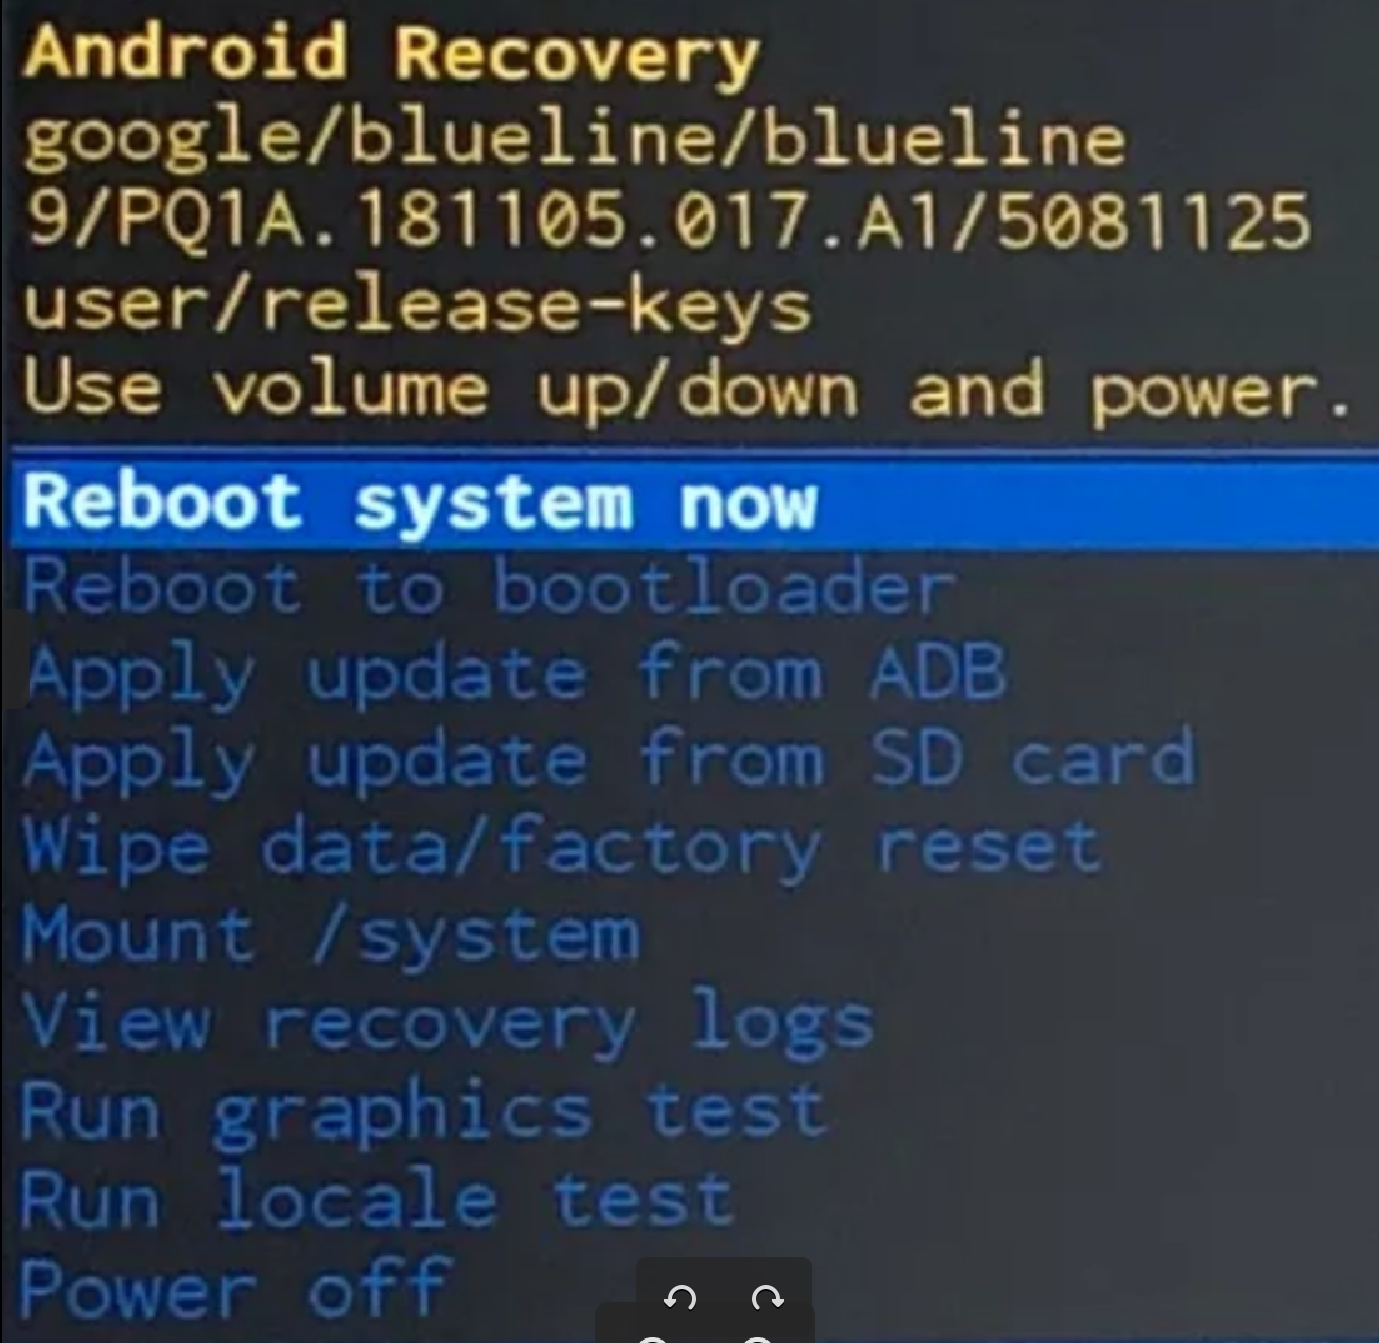
\includegraphics[width=0.5\columnwidth]{images/recovery.png}
    \caption{Foto da tela de recuperação de dados de um dispositivo Android.}
    \label{fig:recovery}
\end{figure}

\subsection{Sobrescrita de dados}

Utilizaremos uma distribuição Linux para todo o processo abaixo.

Para realizar a destruição de dados, primeiro precisamos explorar as partições do nosso dispositivo para identificar onde os dados que desejamos explorar estão armazenados. Para isso, temos algumas opções.

Primeiro, precisamos habilitar o "USB debugging" no dispositivo. Isso é feito em "Developer Options". Para habilitar as "Developer Options", precisamos clicar 7 vezes em "Build Number" em "About Phone".

Com o dispositivo conectado ao computador, podemos tentar acessar as partições diretamente com o comando "fdisk -l". Se o dispositivo permitir, para sobrescrever os dados, basta identificar a maior partição do dispositivo e utilizar uma ferramenta como o "shred" para sobrescrever todos os dados dela.

Possivelmente, o dispositivo não permitirá o acesso direto às partições. Nesse caso, podemos utilizar o "adb" para acessar o dispositivo. Para isso, precisamos instalar o "adb" no computador e, com o "adb" instalado, podemos acessar o dispositivo usando o comando "adb shell".

Através do "adb", podemos navegar pelas partições do dispositivo e identificar onde os dados que desejamos sobrescrever estão armazenados.

O "adb" também permite que utilizemos ferramentas do nosso sistema no dispositivo Android. Para isso, basta executar, por exemplo, o comando "adb shell "su -c 'dd if=/dev/block/mmcblk0'".

Com acesso às partições, podemos utilizar a ferramenta de nossa preferência para realizar a sobrescrita dos dados.

Outra alternativa é a ferramenta "jmptfs"; alguns dispositivos serão reconhecidos como um dispositivo "MTP" ao invés de um dispositivo de armazenamento externo. Nesse caso, podemos utilizar o comando "jmptfs ~/pasta\_de\_destino" para montar o dispositivo e acessar as partições.